\chapter{Nodes}
If one were to ask a random group of people to draw a network on a piece of paper, it is likely that most would draw dots to represent the nodes, and lines joining the dots to represent the edges. This is a representation so intuitive that it is often synonymous with the abstract concept of a network entirely.
This is the reason why this `join-the-dots' representation, known as the node-link diagram, is the most commonly studied and applied \cite{Ghoniem2004}, and is also why it has been chosen for the purposes of this thesis.

However it is useful to have an idea of the other possible representations in order to gain a broader view of what network visualisation entails. A classical example of this includes the \emph{matrix plot}, which is a grid where each vertex is represented by a row and a column, and each edge is a dot filled in at the intersection of a row and column \cite{Liiv2010}.
A more obscure example is \emph{string graphs}, where each vertex is represented by a (possibly curved) line, and edges exist between vertices whose lines intersect.
Specialised types of networks can also have similarly specialised representations. Trees, for example, can be depicted as packed rectangles \cite{Johnson1991} or circles \cite{Wang2006}.
Graphs with low \emph{boxicity}, such as food webs \cite{Eklof2013}, can be drawn as \emph{intersection graphs} of overlapping lines or rectangles or cuboids.\footnote{Or hypercuboids, although the usefulness of that for visualisation is likely limited.}
A related and more common example is the \emph{disc graph}, where nodes are represented by circles and edges exist if the circles overlap. This sees widespread use as a Venn diagram, but usually without the connotation of network structure.
A gallery of such examples can be seen in Figure~\ref{fig:graph_representations}. Because of the difference between the abstract mathematical structure of a network and its representation within a visualisation, the abstract structure itself will henceforth be refered to a graph comprised of vertices and edges, and its representation a a network comprised of nodes and links.\footnote{This is in line with the terminology chosen by the \emph{International Symposium on Graph Drawing and Network Visualisation} to separate its theoretical and applied submission tracks, and so I will attempt to adopt it here. However the distinction between the two can sometimes become blurred depending on the context.}

\begin{figure}
\caption[A gallery of graph representations]{Each of these representations has its unique benefits and downsides. Matrix plots can show a very dense amount of data in a small space, but are very dependent on the ordering of rows and columns \cite{Liiv2010}.
The intersection-style graphs are intuitive, but cannot be drawn for all graphs \cite{TODO}.}
write something about treemaps
\label{fig:graph_representations}
\end{figure}

Even within the subfield of node-link diagrams, there is a wide variety of options available.
Examples include \emph{arc} or \emph{chord diagrams}, where nodes are placed on a line or around a circle, respectively. Links are then added by drawing the eponymous arcs or chords between nodes.
A method that has recently gained popularity is the \emph{hive plot}, a simple but effective variant of parallel coordinate plots \cite{Krzywinski2012}, which places nodes on radial lines to draw curves between them, in a similar fashion to radar charts \cite{Porter2018}. An important subtlety is that each node may or may not be placed on more than one line, and the order in which the nodes are spread across the line is also a conscious choice. This customisability is where the power of such a method lies.

Hopefully the above examples give a taste of how varied the representation of a network can be. In this chapter we will focus on... TODO
% """
%  From the 1980s, industrial demand for graph drawing algorithms has grown
% – Software engineering: CASE systems, reverse engineering – Biology: PPI networks, gene regulatory networks
% – Physical networks: network management tools
% – Security: risk management, money movements
% – Social network analysis
% – Customer relationship management: value identification Many companies buy graph drawing algorithms, many code them.
% Currently the international market for graph drawing algorithms is in the hundreds of millions of dollars per year.
% """

\section{Background}
\label{sec:nodes_background}
The formal study of node-link diagrams dates back to least the 1920s. For example, F\'ary's theorem is a famous proof that any planar graph, defined as a graph that can be drawn without any intersecting links, can always be drawn in a planar way without needing links to be curved. This proof is attributed to F\'ary who published it in 1948 \cite{Fary1948}, and was independently discovered by a host of other authors in the same era \cite{Steinitz1922, Wagner1936, Koebe1936, Stein1951}.
The ensuing development of actual \emph{algorithms} for network layout emerged around the 1960s, with its seminal work widely attributed to the barycentre algorithm of Tutte in 1963 \cite{Tutte1963}. 

Tutte's algorithm is very simple, and boils down to solving a system of linear equations, each of which strives to set a single node to the barycentre (i.e.\ mean position) of its neighbours. This is defined as 
\begin{equation}
  \mathbf{X}_i = \frac{1}{|N(i)|}\sum_{j\in N(i)}\mathbf{X}_j
\label{eq:tutte}
\end{equation}
where $\mathbf{X}_i$ is the $i^\text{th}$ row of the $|V|\times k$ matrix $\mathbf{X}$, with $V$ being the set of vertices in the graph and $k$ the dimensionality of the layout (usually two); $N(i)$ is the set of vertices neighbouring $i$.
Throughout this chapter, $\mathbf{X}$ will represent the coordinates of nodes in a layout.
Note that a necessary initial step is to fix the position of a selection of nodes around the boundary of the drawing, in order to avoid the trivial solution of placing all nodes in the same position.
The powerful insight that Tutte revealed with his algorithm was a remarkable mathematical theorem attached to it. He proved that this barycentre algorithm will always produce a planar drawing, in the specific case that the graph is planar and tri-connected (i.e.\ the graph cannot be disconnected by removing two vertices, no matter which two are removed).

This algorithm has served as the springboard for two main branches of network layout algorithms. Since planarity has been shown to be one of, if not the most important markers for readability in node-link diagrams \cite{Purchase1997}, the first branch is a line of planarity-based algorithms which can guarantee planar node layouts. Examples include the algorithm of Read \cite{Read1987} which recursively removes nodes and adds dummy edges to maintain a triangulated graph at each step.  A problem with this method and Tutte's is \emph{node resolution}, which means that nodes may be placed exponentially close to each other, rendering the graph impossible to read in certain areas.
A breakthrough for this problem came in 1990 by de Fraysseix et al.\ \cite{DeFraysseix1990} who described the first layout algorithm achieve an asymptotically optimal node resolution of being able to layout nodes on an $\mathcal{O}(|V|\times |V|)$ grid and in linear time \cite{Chrobak1995}. This was done by constructing a \emph{canonical ordering} of the graph \cite{Zhang2005} which is used to order nodes on the x-axis, and from there y-axis positions can be chosen such to avoid crossings.
Improvements and refinements have been made with this algorithm in mind \cite{Zhang2005}, but none have managed to solve the problem of poor \emph{angular resolution}, which means that adjacent edges form small angles between each other, another property that has been shown to impact the readability of layouts \cite{Purchase1997}.
This issue exists until this day \cite{Eades2012}, and is a primary reason why most network visualisation software uses algorithms based on a second, less mathematically rigorous branch of algorithms inspired by Tutte.

This second branch comes from an intuitive interpretation of Tutte's algorithm: that each edge is analogous to a spring of natural length 0, where the solution to Tutte's system of linear equations can be seen as the point at which the elastic energy of these springs, according to Hooke's law \cite{Hooke1678}, is minimised. This energy is defined as
\begin{equation}
  \mathrm{energy}(\mathbf{X}) = \sum_{\{i,j\}\in E}||\mathbf{X}_j-\mathbf{X}_i||^2
\label{eq:tutte_energy}
\end{equation}
where $E$ is the set of all edges. Differentiating with respect to the position of a single node $\mathbf{X}_i$ results in
\begin{equation}
  \frac{d}{d\mathbf{X}_i}\mathrm{energy}(\mathbf{X}) = \sum_{j\in N(i)}-2(\mathbf{X}_j-\mathbf{X}_i)
\label{eq:tutte_force}
\end{equation}
where it can be seen that setting the left-hand side to zero results in Equation~\eqref{eq:tutte}, corresponding to an embedding of minimum global energy in the system.

This interpretation has been taken and advanced to alleviate the resolution problem present in planarity based methods, by introducing the trade-off of foregoing mathematical rigour. 
This is done by using human intuition to formulate variations on Equation~\eqref{eq:tutte_energy}, in what are known as \emph{force-directed} algorithms.

\subsection{\texorpdfstring{\st{Force-directed}{ Optimisation algorithms}}{}}
\label{sec:force_background}
This section will present an overview of the various methods that have been sprouted from this second branch of algorithms, around which the work in this chapter is based. All such algorithms will also be framed within the wider context of \emph{optimisation}, a framework which will tie together otherwise loosely-connected threads in a logical taxonomy.
It will also lead more cogently into the novel contributions described in Section~\ref{sec:sgd}.

\begin{figure}
  \caption[A gallery of node layout methods]{A binary tree of depth TODO visualised using some of the algorithms described in Section~\ref{sec:force_background}. The corresponding equations from left to right are: Tutte~\eqref{eq:tutte}, Eades~\eqref{eq:eades}, spectral~\eqref{eq:spectral}, and stress~\eqref{eq:stress}. Note that...}
  \label{fig:misc_force_layouts}
\end{figure}

The earliest of these algorithms was developed in 1984 by Eades \cite{Eades1984} who, inspired by techniques for positioning transistors on integrated circuits \cite{Quinn1979}, made two modifications. The first was to alter the edge springs in order to give them a non-zero natural length, avoiding having to fix an often arbitrary selection of nodes around the boundary. The second was to introduce a repulsive force between pairs of non-adjacent vertices to spread nodes evenly around the drawing.
The combination of these forces on a single node $i$ is defined as
\begin{equation}
  \frac{d}{d\mathbf{X}_i}\mathrm{energy}(\mathbf{X}) = -\sum_{j\in N(i)}c_1\log(||\mathbf{X}_j-\mathbf{X}_i||)\overrightarrow{\mathbf{X}_{ij}}
  + \sum_{j\notin N(i)}\frac{c_2}{||\mathbf{X}_j-\mathbf{X}_i||^2}\overrightarrow{\mathbf{X}_{ij}}
  \label{eq:eades}
\end{equation}
where $\overrightarrow{\mathbf{X}_{ij}} = \frac{\mathbf{X}_j-\mathbf{X}_i}{||\mathbf{X}_j-\mathbf{X}_i||}$, i.e.\ the normalised vector pointing from $i$ to $j$, and $c_1$ and $c_2$ are constant parameters determining the relative strengths of the forces. The first summation defines the `springs', where the logarithm attempts to maintain the spring at unit length by flipping to negative if the node pair gets too close together.\footnote{Hooke's law was abandoned by Eades because ``\emph{Experience shows that Hookes Law (linear) springs are too strong when the vertices are far apart; the logarithmic force solves this problem}" \cite{Eades1984}.}
The second summation is the repulsive force, which always pushes $i$ away from $j$ if there does not exist an edge between them, and decays according to an inverse square function analogous to charged electrons obeying Coulomb's law \cite{Coulomb1785}.

There are two important aspects to notice here. The first is that the left-hand side is not the energy itself, but its derivative. The second is that this derivative can no longer be straightforwardly solved as in Equation~\eqref{eq:tutte} because it has become \emph{non-linear}. How then is energy minimised? Through a method known as \emph{gradient descent}, which is as simple as iteratively moving nodes in the direction opposite to the derivative in Equation~\eqref{eq:eades} according to
\begin{equation}
  \mathbf{X}_i \leftarrow -\eta\, \frac{d}{d\mathbf{X}_i}\mathrm{energy}(\mathbf{X})
\label{eq:gradient_descent}
\end{equation}
where $\eta$ is a constant parameter.
This operation, despite its simplicity, is theoretically proven to find a minimal energy embedding \cite{Cauchy1847}, although it is important to note that this embedding may not be globally optimal because the energy function defined by~\eqref{eq:eades} is \emph{non-convex} and therefore may contain many \emph{local minima}. Many of the concepts introduced in this paragraph will be elaborated upon in Section~\ref{sec:stress_background}.

This optimisation through gradient descent interpretation is not how this type of algorithm is commonly presented, as  force-directed algorithms are often categorised into two families: force-balancing and energy-minimising models \cite{Ortmann2017, Brandes2001}.
Eades' model fits into the former, while others fit into the latter by directly defining an energy function such as in~\eqref{eq:tutte_energy}.
Energy is then minimised by gradient descent as in Equation~\eqref{eq:gradient_descent} or by another optimisation technique, as will be further elaborated upon in Section~\ref{sec:stress_background}.
With the view that the action of `force-balancing' is equivalent to gradient descent on another energy function, however, it is made clear that the two families are equivalent in the sense that both strive for the same goal: minimising energy.

This optimisation-centric viewpoint also allows a variety of linear algebra-based methods to be grouped into the same taxonomy.
The algorithm of Harel and Koren \cite{Harel2004} first embeds a graph in a high-dimensional space, determined by a covariance matrix of graph-theoretic or shortest-path distances, and then finds an optimal projection down to two dimensions by finding the eigenvectors of this this matrix. This is commonly known as principal components analysis (PCA) \cite{Pearson1901}.
The \emph{classical scaling} approach of Brandes and Pich \cite{Brandes2007} is based on constructing the high-dimensional embedding from a double centered \emph{distance matrix} between high-dimensional points and then performing PCA. The intuition behind this method is that it optimises the inner product between low- and high-dimensional distances.
The \emph{Spectral} approach, originally developed by Hall in 1970 \cite{Hall1970} and largely ignored by the field until Koren in 2003 \cite{Koren2003}, uses a graph Laplacian as the high-dimensional matrix instead of shortest-paths, upon which PCA is again applied. This approach is particularly closely related to Tutte's algorithm, which in fact utilises the same graph Laplacian when solving for Equation~\eqref{eq:tutte}.
The eigenvalue approach even optimises the same energy function, but requires the variance of the embedding to be non-zero, thereby avoiding the need to fix certain nodes around the boundary \cite{Koren2003}.
In mathematical terms, its energy upon a single dimension of the layout in the column vector $\mathbf{x}$ can be derived as
\begin{align}
\begin{split}
  \mathrm{energy}(\mathbf{x}) &= \sum_{\{i,j\}\in E}w_{ij}(\mathbf{x}_j-\mathbf{x}_i)^2\\
  \mathrm{var}(\mathbf{x}) &= \frac{1}{n}\sum_i(\mathbf{x}_i-\overline{\mathbf{x}})^2 = 1
\end{split}
\label{eq:spectral}
\end{align}
where $w_{ij}$ is an optional weight given to each edge (previously all set to 1 in~\eqref{eq:tutte}) and $\overline{\mathbf{x}}$ is the mean of $\mathbf{x}$. The one-dimensional layout that minimises energy is equal to the second smallest eigenvector of the Laplacian matrix $\mathbf{L}$, defined such that
\begin{equation}
  \mathbf{x}^T\mathbf{Lx} = \mathrm{energy}(\mathbf{x})
\end{equation}
where $\mathbf{x}^T$ denotes the transpose of $\mathbf{x}$. Subsequent dimensions are found by calculating subsequent eigenvectors of $\mathbf{L}$, often through power iteration \cite{Koren2003}.
All of these methods boil down to finding the eigendecomposition of a certain matrix which describes the graph in a different way, and each set of eigenvectors describes an \emph{optimal projection} into a lower dimension.

The linear nature of such methods is a double-edged sword, as it allows them to be calculated and/or approximated quickly and precisely, but they all suffer from the same issue that resulting layouts under-represent local detail \cite{Brandes2009}, especially in examples such as the binary tree in Figure~\ref{fig:misc_force_layouts}. However their effectiveness at capturing global structure consistently has led to them being commonly used as an initialisation step \cite{Brandes2009, Dwyer2009}.

Circling back to non-linear methods, there have been many attempts at improving Eades' original formulation. A widely-used alternative, developed in 1991, is the method of Fruch\-terman and Reingold \cite{Fruchterman1991} who revert springs back to having a natural length of zero, but balance this out by applying the repulsive force between all pairs of vertices. Counter-intuitively, increasing the number of repulsive terms also makes the summation more efficient to calculate, by taking inspiration from techniques used in physical simulations \cite{Hachul2005, Hu2005}. More detail on scaling layout algorithms to large graphs can be found in Section~\ref{sec:large_graphs}.
Another notable attempt came from Frick et al.\ \cite{Frick1995} in 1995, who altered the calculations to never require a square root operation, and introduced a number of extra heuristics to speed up the convergence of the optimisation procedure in Equation~\eqref{eq:gradient_descent}. These heuristics were introduced on an intuitive and ad hoc basis, but have been shown to greatly speed up convergence in practice \cite{Brandes2001}.
% \begin{equation}
%   \frac{d}{d\mathbf{X}_i}\mathrm{energy}(\mathbf{X}) = -\sum_{j\in N(i)}\frac{c^2}{||\mathbf{X}_j-\mathbf{X}_i||}\overrightarrow{\mathbf{X}_{ij}}
%   + \sum_{j:j\neq i}\frac{||\mathbf{X}_j-\mathbf{X}_i||^2}{c}\overrightarrow{\mathbf{X}_{ij}}
% \end{equation}

The energy function that will become the focus for the rest of this chapter is known as \emph{stress}, and was popularised within the context of graph layout in 1989 by Kamada and Kawai \cite{Kamada1989}. Its energy is defined as
\begin{equation}
  \mathrm{stress}(\mathbf{X}) = \sum_{\{i,j\}:i<j}w_{ij}(||\mathbf{X}_j-\mathbf{X}_i||-d_{ij})^2
\label{eq:stress}
\end{equation}
where $w_{ij}$ and $d_{ij}$ are constants specific to each term in the summation. The intuition behind this formulation is that there are Hooke's law springs attached between all pairs of vertices, not just those connected by edges. Each of these springs is of natural length $d_{ij}$ and of stiffness $w_{ij}$. In practice, $d_{ij}$ is usually set to the shortest-path distance between vertices, and $w_{ij}$ is almost always set to $d_{ij}^{\text{--}2}$ in order to suppress the contribution from long-range springs that would otherwise obfuscate local detail \cite{Brandes2009}.

The derivative of this equation is non-linear, like Equation~\eqref{eq:eades} or in \cite{Fruchterman1991, Frick1995}, and so cannot be solved exactly using linear solvers as for Equations~\eqref{eq:tutte_energy} or~\eqref{eq:spectral}.
% However an immediate benefit to this formulation is that there are no extra input parameters for the user to decide, since $w_{ij}$ and $d_{ij}$ are both dependent on the structure of the graph itself.
However, stress as an energy function is known to produce high-quality layouts \cite{Brandes2009}. This is partly because it manages to avoid the \emph{peripheral effect} \cite{Hu2005}, a common visual artifact of many force-directed methods where repulsive forces tend to push nodes towards the boundary of the layout. This can be seen in Figure~\ref{fig:misc_force_layouts}, TODO Position, where the nodes of the tree are TODO. Stress avoids this by forgoing repulsive forces entirely in Equation~\eqref{eq:stress}.

Stress also does not require extra input parameters such as those in Equation~\eqref{eq:eades} because $d_{ij}$ and $w_{ij}$ are both derived from the structure of the graph itself.
However, it is known to be difficult to optimise due to an abundance of local minima \cite{DeLeeuw1988, Gansner2004}, and also does not scale well to larger graphs due to the quadratic number of terms in the summation \cite{Brandes2009, Hu2005}.
The subsequent content of this chapter will aim at addressing these issues through the application of an algorithm known as \emph{stochastic gradient descent} to minimise Equation~\eqref{eq:stress}. Before describing the algorithm itself however, a history of other methods used to minimise stress will first be outlined.

% """
% Force-directed methods account for 90\% of commercial and free graph drawing software for undirected graphs \cite{eades_revisited}
% """
% this is because they are intuitive and easily modified to include domain-specific features \cite{magnets and shit}.

\subsection{Multidimensional scaling}
\label{sec:stress_background}
% Before explaining the details of SGD, I will first outline the history of methods used to optimise Equation~\eqref{eq:stress}, as the performance of SGD will be evaluated through an experimental study comparing it to the previous state-of-the-art, known as \emph{majorization}.
Equation~\eqref{eq:stress} was first utilised in a domain unrelated to graphs, but still for the purpose of visualisation, known as \emph{multidimensional scaling} (MDS). As the name implies, this involves taking high-dimensional data and scaling it down to fewer dimensions, usually two.
The difficulty in this task can be illustrated through a simple example: the humble tetrahedron. The task at hand is to find an `ideal' drawing of the tetrahedron, where `ideal' is defined as having each of its edges drawn with equal length. When one tries to draw such a configuration on a piece of (two-dimensional) paper, it quickly becomes clear that it is not possible.
Even for such a small graph with only four vertices, there are too few dimensions available to provide sufficient degrees of freedom.\footnote{The rate at which such a problem can get out of hand is known as the \emph{curse of dimensionality} \cite{Friedman2001}, which is range of phenomena caused by the exponential growth of a given problem space relative to each additional input dimension}
The next logical question is: what layout gets as close as possible to this ideal?

Multidimensional scaling (MDS) is a technique to solve exactly this type of problem, that attempts to minimize the disparity between ideal and low-dimensional distances.
% but generalized to any number of input or output dimensions.
This is done by defining an equation to quantify the error in a layout, and then minimizing it. While this equation comes in many forms \cite{Cox2000}, stress as in Equation~\eqref{eq:stress} is the most commonly used for graph layout \cite{Brandes2009}, for the reasons described at the end of the previous section.

The use of Equation~\eqref{eq:stress} was popularized for graph layout by Kamada and Kawai \cite{Kamada1989} who minimized the function using a localized 2D Newton-Raphson method, while within the MDS community Kruskal \cite{Kruskal1964a} originally used gradient descent \cite{Kruskal1964}. This was later improved upon by De Leeuw \cite{DeLeeuw1988} with a method known as \emph{majorization},
which minimizes a complicated function by iteratively finding the 
true minima of a series of simpler functions, each of which touches the 
original function and is an upper bound for it \cite{Cox2000}.
This was applied to graph layout by Gansner et al.\ \cite{Gansner2004} and has been the state-of-the-art for the past decade.

\subsection{Majorization}
Majorization is the algorithm that will be used throughout this chapter as the benchmark against which the performance of SGD will be assessed.
It works by first finding a Laplacian matrix $\mathbf{L}^w$, defined as
\begin{equation}
  \mathbf{L}_{ij}^w =
  \begin{cases}
    \;-w_{ij} & \text{if }\;i\neq j\\
    \;-\sum_{k\neq i}\mathbf{L}_{ik}^w & \text{if }\;i=j
  \end{cases}
\end{equation}
and another Laplacian matrix $\mathbf{L^X}$, defined as
\begin{equation}
  \mathbf{L}_{ij}^\mathbf{X} =
  \begin{cases}
    \;-w_{ij}d_{ij}||\mathbf{X}_i-\mathbf{X}_j||^{-1} & \text{if }\;i\neq j\\
    \;-\sum_{k\neq i}\mathbf{L}_{ik}^\mathbf{X} & \text{if }\;i=j.
  \end{cases}
\end{equation}
It can be shown that the equation
\begin{equation}
  \mathbf{L}^w\mathbf{x}' = \mathbf{L^Xx}
  \label{eq:major_linear}
\end{equation}
where $\mathbf{x}$ and $\mathbf{x}'$ are column vectors that represent a single dimension of the full layouts $\mathbf{X}$ and $\mathbf{X}'$ respectively, guarantees that $\text{stress}(\mathbf{X}') \leq \text{stress}(\mathbf{X})$ \cite{Gansner2004}.
The optimisation process is then performed simply by solving Equation~\eqref{eq:major_linear} as a system of linear equations, with $\mathbf{x}'$ as the column of unknowns being solved for. This is repeated in an iterative manner, where $\mathbf{x}'$ is computed in one iteration and then used as $\mathbf{x}\leftarrow\mathbf{x}'$ in the next, until the algorithm can no longer improve the value of stress by more than a certain threshold. Note that $\mathbf{L}^w$ only needs to be computed once, but $\mathbf{L}_{ij}^\mathbf{X}$ must be recalculated on every iteration.

Additionally in practice, the position of the first vertex is fixed to the origin, and the first row and column of $\mathbf{L}^w$ are removed, as well as the first row of the vector $\mathbf{L^X}$. This is in order to remove translational invariance from the solution, which allows for fast linear equation solving methods to be applied to solve Equation~\ref{eq:major_linear}.
In particular, Gansner et al.\ \cite{Gansner2004} recommend \emph{Cholesky factorization} \cite{Press2007a} or the \emph{conjugate gradient} method \cite{Press2007}, both of which will be tested later in Section~\ref{sec:sgd_experiment}. 
Ganser et al.\ \cite{Gansner2004} also described another \emph{local} method for solving Equation~\ref{eq:major_linear}, where the system of equations is solved for just one vertex at a time. This is done by setting the position of vertex $i$ to
\begin{equation}
  \mathbf{x}_i' = \frac{\sum_{j\neq i}w_{ij}(\mathbf{x}_j + d_{ij}(\mathbf{x}_i - \mathbf{x}_j)||\mathbf{X}_i - \mathbf{X}_j||^{-1})}{\sum_{j\neq i}w_{ij}}
  \label{eq:major_local}
\end{equation}
and is also guaranteed to monotonically decrease stress \cite{Gansner2004}. This local method will also be tested in Section~\ref{sec:sgd_experiment}, and will furthermore be important when considering large graphs in Section~\ref{sec:large_graphs}.

\section{Stochastic gradient descent}
\label{sec:sgd}
The remaining content of this chapter will describe the application of stochastic gradient descent (SGD) to minimise stress. SGD is a method widely used in other fields, most notably in machine learning \cite{Bottou2012}, but not previously applied to minimise Equation~\ref{eq:stress}. 
SGD approximates the gradient of a sum of functions using the gradient of its individual terms. For stress in particular, this has an intuitive geometric interpretation of moving a single pair of vertices at a time; this interpretation allows for a simple modification to the optimisation step which help to avoid local minima and speed up convergence (described in Section~\ref{sec:sgd_description}). The benefits of SGD over majorization will be shown through experiment.

\subsection{Constraint relaxation}
\label{sec:wcr_story}
The origin of the work in this chapter is rooted in constrained graph layout, where a relaxation algorithm, here referred to as \emph{constraint relaxation} has gained popularity due to its simplicity and versatility \cite{Dwyer2009,Bostock2011}. This algorithm will provide the context to the geometric interpretation of SGD that will be leveraged to make the modifications in Section~\ref{sec:sgd_description}.

Constraint relaxation was first introduced in video game engines as a technique to quickly approximate the behavior of cloth, which is modeled as a planar mesh of vertices that maintains its edges at a fixed length.
A full physics simulation would represent each edge as a stiff spring, summing up and integrating over the resulting forces, but a realistic piece of cloth contains too many edges for this to be feasible.
To avoid this bottleneck, Jakobsen \cite{Jakobsen2001} introduced the idea of considering each edge independently, moving a single pair of vertices at a time.
While this is a rather simple and perhaps naive idea, in practice the solution converges in very few iterations.

This was utilized by Dwyer \cite{Dwyer2009}, who used the method in conjunction with any standard force-directed layout to achieve effects such as making edges point downwards, or fixing cycles around the edge of a wheel. To define it properly in the case of maintaining a distance $d_{ij}$ between the coordinates of two nodes $\mathbf{X}_i$ and $\mathbf{X}_j$, this \emph{constraint} can be written as
\begin{equation}
  ||\mathbf{X}_i - \mathbf{X}_j|| \leftarrow d_{ij}
  \label{eq:constraint}
\end{equation}
and is \emph{satisfied} by moving $\mathbf{X}_i$ and $\mathbf{X}_j$ in opposite directions by a vector
\begin{equation}
  \mathbf{r} = \frac{||\mathbf{X}_i - \mathbf{X}_j||-d_{ij}}{2}\frac{\mathbf{X}_i - \mathbf{X}_j}{||\mathbf{X}_i - \mathbf{X}_j||}.
  \label{eq:satisfaction}
\end{equation}
This can be seen as a diagram in Figure~\ref{fig:satisfaction}, and is analogous to decompressing an infinitely stiff spring of length $d_{ij}$.
\begin{figure}
  \centering
  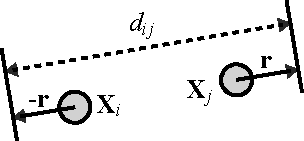
\includegraphics[width=.4\textwidth]{stress/satisfaction.pdf}
  \caption{Satisfaction of the distance constraint described by Equation~\eqref{eq:constraint}.}
  \label{fig:satisfaction}
\end{figure}
Rewriting Equation~\eqref{eq:stress} as
\begin{gather}
\label{stress-terms}
\mathrm{stress}(\mathbf{X}) = \sum_{i<j} Q_{ij}(\mathbf{X}),\\
\label{qij}
Q_{ij}(\mathbf{X}) = w_{ij}(||\mathbf{X}_i - \mathbf{X}_j|| - d_{ij})^2,
\end{gather}
it can be seen that if every term $Q_{ij}$ in the summation is satisfied as a constraint~\eqref{eq:constraint}, then the total stress is zero, corresponding to an ideal layout. 
This is exactly the idea behind the method that will be studied here---a constraint is placed on every possible pair of vertices, and then satisfied one by one as above.

However zero stress is almost always impossible, for the same reasons that the aforementioned tetrahedron cannot be embedded in 2D. In such situations, simply satisfying constraints does not lead to convergence, but a simple extension will now be described that not only converges but, remarkably, also minimises stress.

\subsection{Constraints are terms TBD}
\label{sec:sgd_description}
The modifications required to the constraint relaxation described above can be understood by first noticing that satisfying a constraint is equivalent to moving both vertices in the direction of the gradient of a stress term $Q_{ij}$
\begin{equation}
  \label{gradient}
  \frac{\partial Q_{ij}}{\partial\mathbf{X}_i}=\frac{\partial}{\partial\mathbf{X}_i}w_{ij}(||\mathbf{X}_i - \mathbf{X}_j|| - d_{ij})^2 = 4w_{ij}\mathbf{r}.
\end{equation}
The full gradient $\partial Q_{ij}/\partial\mathbf{X}$ can be written as
\begin{equation}
  \frac{\partial Q_{ij}}{\partial\mathbf{X}_k}=
  \begin{cases}
    \;4w_{ij}\mathbf{r} & \mbox{if $k=i$} \\
    \;-4w_{ij}\mathbf{r} & \mbox{if $k=j$} \\
    \;0 & \mbox{otherwise.} \\
  \end{cases}
\end{equation}
Recall that standard force-directed methods use (non-stochastic) gradient descent, following Equation~\eqref{eq:gradient_descent}, and that this involves taking a step in the opposite direction to the derivative of the entire summation at once.
The change to stochastic gradient descent is as simple as doing the same thing, but to a single term at a time.

Specifically, this involves repeatedly selecting a single term $Q_{ij}$ and applying the iterative formula $\mathbf{X}\leftarrow \mathbf{X}-\eta\nabla Q_{ij}(\mathbf{X})$
Note that since this gradient is zero with respect to all $\mathbf{X}_k$ other than $\mathbf{X}_i$ and $\mathbf{X}_j$, it suffices to update the positions of $\mathbf{X}_i$ and $\mathbf{X}_j$ by
\begin{equation}
  \begin{bmatrix}\mathbf{X}_i\\\mathbf{X}_j\end{bmatrix}
  \leftarrow
  \begin{bmatrix}\mathbf{X}_i\\\mathbf{X}_j\end{bmatrix}+
  \begin{bmatrix}\Delta \mathbf{X}_i\\\Delta \mathbf{X}_j\end{bmatrix}
  =
  \begin{bmatrix}\mathbf{X}_i\\\mathbf{X}_j\end{bmatrix}-
  4w_{ij}\eta
  \begin{bmatrix}\mathbf{r}\\-\mathbf{r}\end{bmatrix}.
  \label{eq:SGD_step}
\end{equation}

The constraint relaxation of the previous section is therefore equivalent to a special case of SGD where $w_{ij}=1$ and $\eta=1/4$.\footnote{The equivalence stochastic gradient descent was not known for a long time, as neither Jakobsen \cite{Jakobsen2001} nor Dwyer \cite{Dwyer2009} classified the algorithm correctly. In fact, not even we knew that this was SGD in the first version of this paper we submitted to a journal.}
Note that a gradual reduction in $\eta$ is necessary to make the process converge, since not all terms can be simultaneously minimised. This can be interpreted here as each edge of the aforementioned tetrahedron satisfying its constraint one by one as in Figure~\ref{fig:satisfaction}, but never finding a configuration where all are satisfied at the same time.

KEEP GOING FROM HERE TOMORRWO
Writing $\mu=4w_{ij}\eta$ as the coefficient of $\mathbf{r}$, it can be seen that $Q_{ij}\leftarrow 0$ when $\mu=1$ and decreases monotonically from $\mu=0$ to $\mu=1$.
Since we have this extra geometric structure that is not normally available in SGD settings, we investigated a modified SGD algorithm in which we set a hard upper limit of $\mu\leq 1$:
\begin{equation}
  \begin{aligned}
    \Delta\mathbf{X}_i &= -\Delta\mathbf{X}_j = -\mu\, \mathbf{r},\\
    \mu&=\min\{\,w_{ij}\eta, \, 1\,\}
  \end{aligned}
  \label{mu}
\end{equation}
where the constant factor $4$ has been removed to...
This modified algorithm makes updates that are identical to standard SGD when $\eta$ is sufficiently small,
\begin{equation}
  % \eta<1/\max_{ij} w_{ij}.
  \eta<\frac{1}{w_{\max}}.
  \label{eta-sufficiently-small}
\end{equation}
Since this will always eventually be the case, it has the same asymptotic convergence properties as standard SGD, which we discuss in Section~\ref{unlimited iterations}.
However, we find that introducing this upper limit on $\mu$ allows for much larger initial step sizes than standard SGD,
yielding much faster convergence without getting stuck in local minima. We show by experiment that this is true for a wide range of graphs (except for a single specific case, see Section~\ref{quality}).
In addition, we use random reshuffling of terms unless otherwise stated (see Section~\ref{randomization}). We define a full pass through all the terms $Q_{ij}$ as a single \emph{iteration}, while a single application of Equation~(\ref{SGD step}) will be known as a \emph{step}.
From now on, we will refer to our modified SGD algorithm simply as SGD.

Plots of stress achieved using SGD compared to majorization are presented briefly in Figure~\ref{stress plots}, and in more detail in Section~\ref{results}. Pseudocode is shown in Algorithm~\ref{pseudocode} (Figure~\ref{algorithm1}).
All results in this paper have vertex positions initialized uniformly randomly within a 1$\times$1 square.
Unless stated otherwise, graph data is from the SuiteSparse Matrix Collection~\cite{davis2011university}. Tests were performed using C\# running in Visual Studio, on an Intel Core i7-4790 CPU with 16GB of RAM.

\begin{figure}
    \centering
    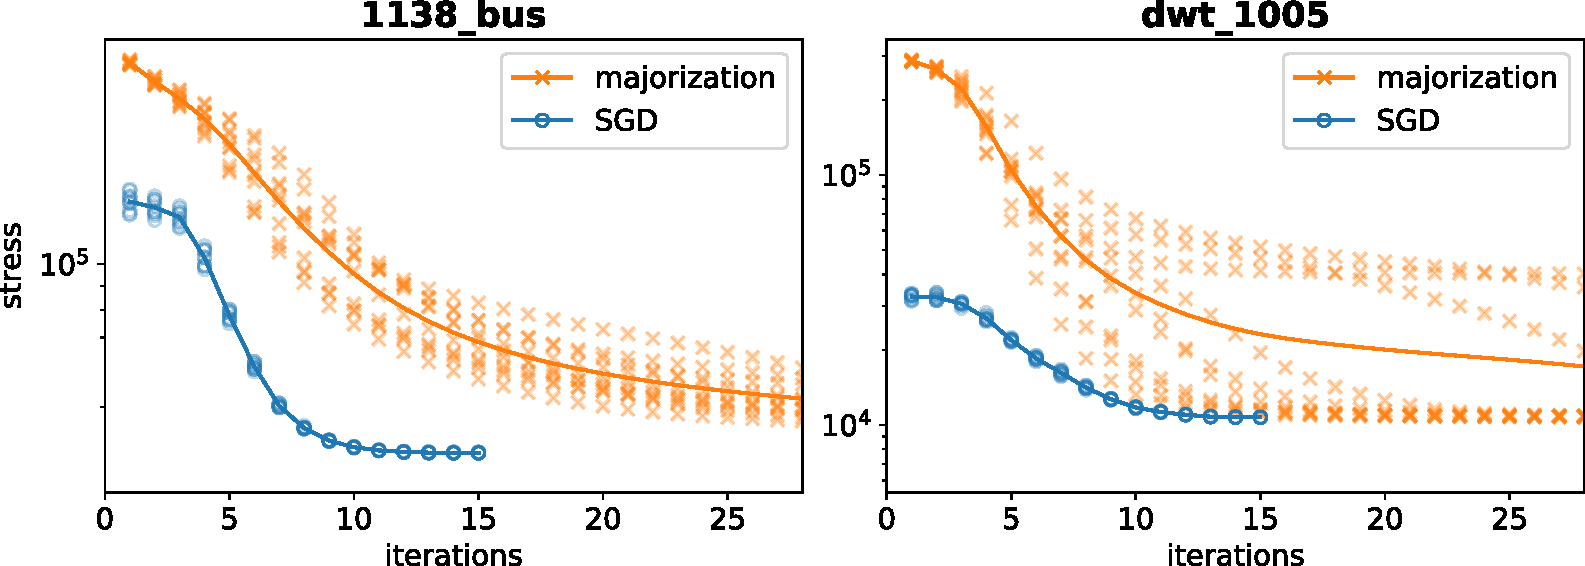
\includegraphics[width=.9\linewidth]{stress/iterations.pdf}
    \caption{Plots of stress for SGD and majorization on the graphs \texttt{1138\_bus} and \texttt{dwt\_1005}, each initialized randomly within a 1$\times$1 square.
    The circles and crosses show stress on each iteration over 10 runs, with the line running through the mean.
    Initial stress values are omitted.
    SGD is clearly more consistent, always reaching lower stress levels than majorization ever manages in hundreds of iterations on \texttt{1138\_bus}.
    They both reach the same overall minimum on the more mesh-like \texttt{dwt\_1005}, but majorization often gets stuck on a particularly dangerous local minimum, shown by its diverging paths.
    A more detailed timing analysis on a wide variety of other examples can be seen in Section~\ref{sec:sgd_experiment}.
	}
    \label{fig:stress_plots}
\end{figure}

\begin{figure}
  \removeAlgorithmFigureError
  \begin{algorithm}[H]
    \SetKwProg{SGD}{SGD}{}{}
    \SetKwInOut{Input}{inputs}
    \SetKwInOut{Output}{output}
    \SetKwFor{ForEach}{foreach}{:}{}
    \SetKwFor{For}{for}{:}{}
    \SetKwIF{If}{ElseIf}{Else}{if}{:}{elif}{else}{}
    
    \SGD{\emph{\textbf{(}}$G$\emph{\textbf{):}}}{
        \Input{graph $G=(V,E)$}
        \Output{$k$-dimensional layout $\mathbf{X}$ with $n$ vertices}
        
        $d_{\{i,j\}} \leftarrow ShortestPaths(G)$
        \label{code:bacon}
        
    %     $w_{\{i,j\}} \leftarrow d_{\{i,j\}}^{-2}$
        
        $\mathbf{X} \leftarrow RandomMatrix(n,k)$
        \label{code:init}
    
    %     $c \leftarrow Max(d)$
        
        \For{$\eta$ in annealing schedule}{
        \label{code:annealing}
        
    %     	$c \leftarrow Cooling(k)
        
            \ForEach{$\{i,j:i<j\}$ in random order}{
    
                $\mu \leftarrow w_{ij} \eta$
                
                \If{$\mu > 1$}{ \label{code:if1}
                    $\mu \leftarrow 1$ \label{code:if2}
                }
                % $\mu \leftarrow Min(w_{ij}\,c\,,\ 2)$
                
    %             $\mathbf{r} \leftarrow \frac{(d_{ij} - ||\mathbf{X}_i - \mathbf{X}_j||)\,(\mathbf{X}_i - \mathbf{X}_j)}{2\,||\mathbf{X}_i - \mathbf{X}_j||}$
                $\mathbf{r} \leftarrow \frac{||\mathbf{X}_i - \mathbf{X}_j||-d_{ij}}{2}\frac{\mathbf{X}_i - \mathbf{X}_j}{||\mathbf{X}_i - \mathbf{X}_j||}$
                
                $\mathbf{X}_i \leftarrow \mathbf{X}_i - \mu\,\mathbf{r}$
                \label{code:satisfaction1}
                
                $\mathbf{X}_j \leftarrow \mathbf{X}_j + \mu\,\mathbf{r}$
                \label{code:satisfaction2}
            }
    %         $c \leftarrow c/2$
        }
    }
    \caption{Stochastic Gradient Descent}
    \label{pseudocode}
  \end{algorithm}

  \caption{
  Pseudocode for the algorithm described in Section~\ref{wcr description}.
  The results in this paper initialize positions randomly within a 1$\times$1 square on line~\ref{pseudo:init}.
  The annealing schedule on line~\ref{pseudo:annealing} is explained in Section~\ref{sec:annealing}.
  }
  \label{algorithm1}
\end{figure}

\subsection{Step size annealing}
\label{sec:annealing}
recall that simply satisfying constraints will not 
finding $\eta_{\max}$ and $\varepsilon$.

\subsection{Randomisation}
random bits

\subsection{SGD vs.\ Majorization}
\label{sec:sgd_experiment}
comparison to majorization


\section{Large graphs}
\label{sec:large_graphs}
various bottlenecks
khoury low rank stress majorization is different from subspace optimisation in graphviz
normal MDS community has some options like Halko et al.\ \cite{TODO} or GLINT, but an additional problem with graphs is that shortest paths still need to be computed, and so we cannot presume that the entire distance matrix is available to us.
multisource shortest paths is still used to find regions
but we present a simpler algorithm to find weights (make pseudocode)
note that it does not really minimise a particular function because the weights are asymmetric.

\subsection{Sparse stress}

\section{Cookbook}
tweaks to the algorithm for various applications
Nails can be used to hold a node in place \cite{something}
Magnetic fields or magnetised springs can be used to align nodes in various ways
Attractive forces can be used to keep clusters together
\subsection{Radial layout}
cool much more than usual for convergence
\subsection{Fixing one dimension}
adding extra initial iterations can help
setting $\mu_{\max}=1.1$ is good too, if not necessary
\subsection{Pinning nodes}
especially good if many are pinned (mention graphviz), because terms can be left out of the summation very easily (unlike majorization), which also means that disconnected components are easily dealt with by never adding those terms (rather than separate solvers for each component).
\subsection{General multidimensional scaling}
show the digits dataset (note that weights are all set to 1)
show lesmis graph
try Phate classical MDS stuff
graphviz optimises in a subspace first?